\chapter{От механики частиц к классическим полям}

\section{Что такое поле}

В предыдущей лекции релятивистская механика частиц выводилась из инвариантного действия. Теперь мы меняем динамический объект. Речь пойдет о классической теории поля, а не о квантовой теории поля. Квантовая механика иногда будет служить полезным сравнением, но уравнения этой главы описывают обычные классические поля. Привычной фоновой моделью служит электромагнетизм: электромагнитные волны распространяются в пространстве и взаимодействуют с заряженными частицами. Мы начнем с еще более простого поля.

Пространство-время может иметь много пространственных координат, но временная координата у него одна. Запишем
\begin{equation}
x^\mu=(t,x^1,\ldots,x^d),
\end{equation}
где пространственный индекс \(i=1,\ldots,d\). Число \(d\) может быть равно трем, как в нашем мире, или одному, двум, девяти, двадцати пяти, либо любому другому значению, полезному в модели. Важная асимметрия на этом этапе состоит в том, что временное направление по-прежнему только одно. Лекция не пытается объяснить, почему теории с несколькими временами столь трудны; она просто принимает схему с одной временной координатой, в которой формулируется обычная причинная физика.

Поле — это измеримая величина, значение которой может меняться от точки к точке и от момента к моменту. Простым примером служит температура:
\begin{equation}
T=T(\mathbf{x},t).
\end{equation}
Она сопоставляет каждому событию одно число, поэтому является скалярным полем. Скорость ветра тоже меняется в пространстве и времени, но имеет величину и направление и потому обладает несколькими компонентами; это векторное поле. В релятивистской физике естественные векторы имеют четыре компоненты, а не три.

В большей части этой лекции поле имеет одну компоненту и обозначается греческой буквой, соответствующей букве \(f\):
\begin{equation}
\phi=\phi(\mathbf{x},t).
\label{eq:sr4-field-definition}
\end{equation}
То, что \(\phi\) называется скаляром, в конечном счете будет означать больше, чем просто наличие одной компоненты. Это будет означать, что все инерциальные наблюдатели приписывают \(\phi\) одно и то же значение в одном и том же физическом событии. Этот закон преобразования появляется лишь после того, как построена вариационная механика.

\section{Частица как прототип}

\subsection{Координата, называемая \texorpdfstring{\(\phi\)}{phi}}

Самый быстрый путь к теории поля начинается с того, что мы возвращаемся к обычной нерелятивистской частице. Пусть частица движется вдоль прямой, но ее координату будем называть \(\phi\), а не \(x\). Нет никакой математической необходимости обозначать координату через \(x\); необычное обозначение выбрано, чтобы сделать наглядной предстоящую аналогию. Отложим время по горизонтали. Тогда вся история частицы представляет собой кривую \(\phi(t)\), которая может проходить через положительные и отрицательные значения.

При фиксированных начальном и конечном моментах времени \(a\) и \(b\) действие имеет вид
\begin{align}
A[\phi]
&=\int_a^b dt\,L(\phi,\dot\phi),\\
L(\phi,\dot\phi)
&=\frac{m}{2}\dot\phi^{\,2}-V(\phi).
\label{eq:sr4-particle-lagrangian}
\end{align}
Уравнение Эйлера--Лагранжа имеет вид
\begin{equation}
\frac{d}{dt}\left(\frac{\partial L}{\partial\dot\phi}\right)
-\frac{\partial L}{\partial\phi}=0.
\label{eq:sr4-particle-el}
\end{equation}
Для лагранжиана из \eqref{eq:sr4-particle-lagrangian}
\begin{equation}
\frac{\partial L}{\partial\dot\phi}=m\dot\phi,
\qquad
\frac{\partial L}{\partial\phi}=-\frac{dV}{d\phi},
\end{equation}
поэтому
\begin{equation}
\boxed{m\ddot\phi=-\frac{dV}{d\phi}}.
\label{eq:sr4-newton}
\end{equation}
Это просто уравнение Ньютона, записанное с \(\phi\) в роли координаты.

\begin{figure}[htbp]
\centering
\includegraphics[width=0.90\textwidth]{lecture_04_figure_01.png}
\caption{Обычное уравнение Эйлера--Лагранжа и его ньютоновский результат для координаты \(\phi(t)\).}
\lectureframe{00:10:18}
\end{figure}

Физическая траектория делает действие стационарным при фиксированных концах. В лекции часто говорится \emph{минимум}, но точное утверждение — стационарность: траектория может давать минимум, максимум или другое стационарное значение. Полезно мысленно разбить интервал времени на множество малых частей. Тогда действие становится функцией множества выбранных значений \(\phi\). Изменение этих значений при фиксированных концах и дифференцирование по каждому из них — конечномерный предок уравнения Эйлера--Лагранжа.

\subsection{Механика как теория в \texorpdfstring{\(0+1\)}{0+1} измерениях}

Теперь представьте мир, в котором есть время, но нет пространственных измерений. Его пространство — одна-единственная точка. Поле в таком мире не может зависеть от положения, потому что нет положения, от которого можно было бы зависеть; оно может быть только функцией \(\phi(t)\). Поэтому обычную механику частицы с одной координатой можно рассматривать как теорию поля в \(0+1\) измерениях. Математика не изменилась. Изменилась только интерпретация: вместо положения частицы речь идет о значении поля в мире без пространства.

\begin{figure}[htbp]
\centering
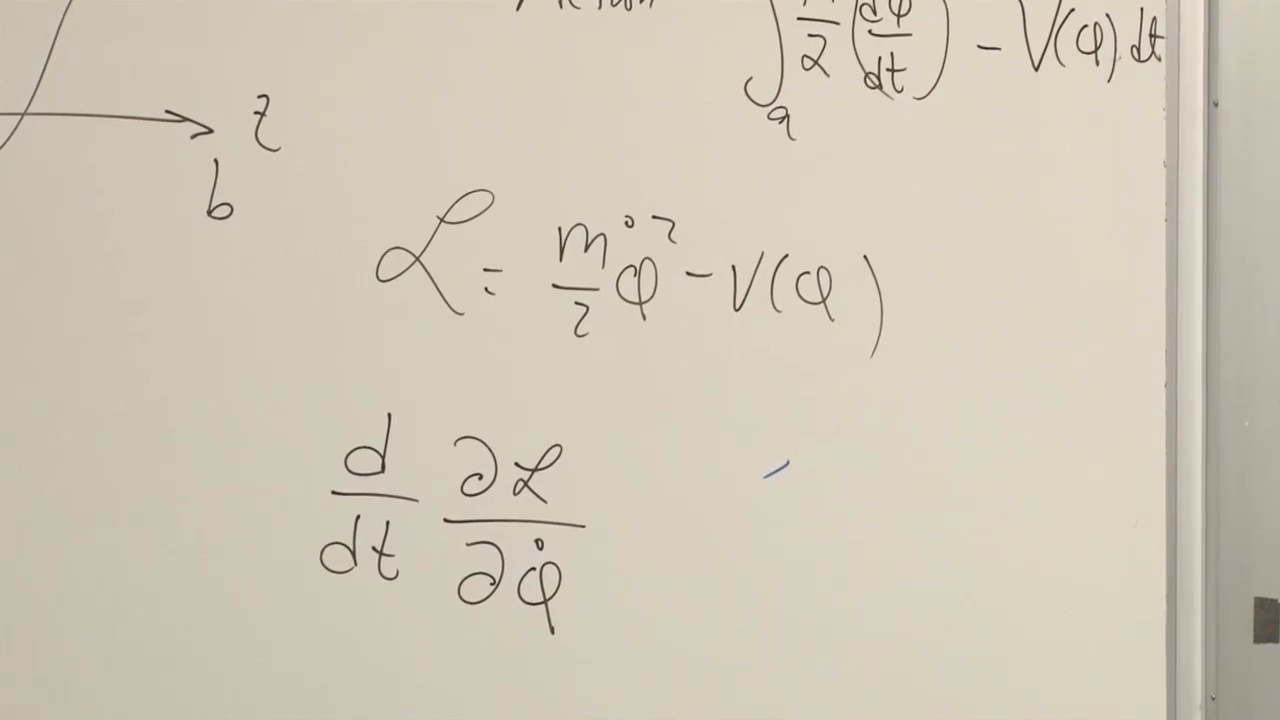
\includegraphics[width=0.90\textwidth]{lecture_04_figure_02.png}
\caption{Дискретизированная история \(\phi(t)\): траектория частицы и, в новой интерпретации, история поля в \(0+1\) измерениях.}
\lectureframe{00:14:30}
\end{figure}

\begin{classroomqa}
\audiencequestion{Исчезает ли потенциал, когда нет пространственных измерений?}
\lecturerresponse{Нет. Пространственная зависимость исчезает, но у поля все равно есть значение. Энергия может зависеть от этого значения через \(V(\phi)\). В интерпретации частицы смещение кривой вверх или вниз меняет потенциальную энергию; в интерпретации поля разные значения \(\phi\) имеют разную потенциальную энергию. \lecturetimestamp{00:15:00}}
\end{classroomqa}

\begin{classroomqa}
\audiencequestion{Вместо того чтобы воображать полное отсутствие пространства, можно ли представить себе обычное пространство, в котором поле зависит только от времени?}
\lecturerresponse{Да. Для этой цели локальная математика одинакова: все пространственные производные исчезают, и остается только \(\phi(t)\). Называя это \(0+1\)-мерной теорией, мы выделяем эту редуцированную структуру, но пространственно однородное поле в большем мире дает ту же интуицию. \lecturetimestamp{00:16:25}}
\end{classroomqa}

Смысл этого обходного пути теперь ясен. Мы знаем принцип действия для поля, зависящего от одной координаты — времени. По этому образцу можно угадать принцип действия для поля, зависящего от всех координат пространства-времени.

\section{История поля в пространстве-времени}

\subsection{От кривой к поверхности}

В \(1+1\) измерениях само пространство-время — это плоскость с координатами \(t\) и \(x\). Значение \(\phi(x,t)\) задает третье направление. Поэтому история поля представляет собой не кривую, а поверхность над плоскостью пространства-времени. Она может подниматься выше нуля или опускаться ниже него, потому что скалярное поле не обязано быть положительным.

\begin{figure}[htbp]
\centering
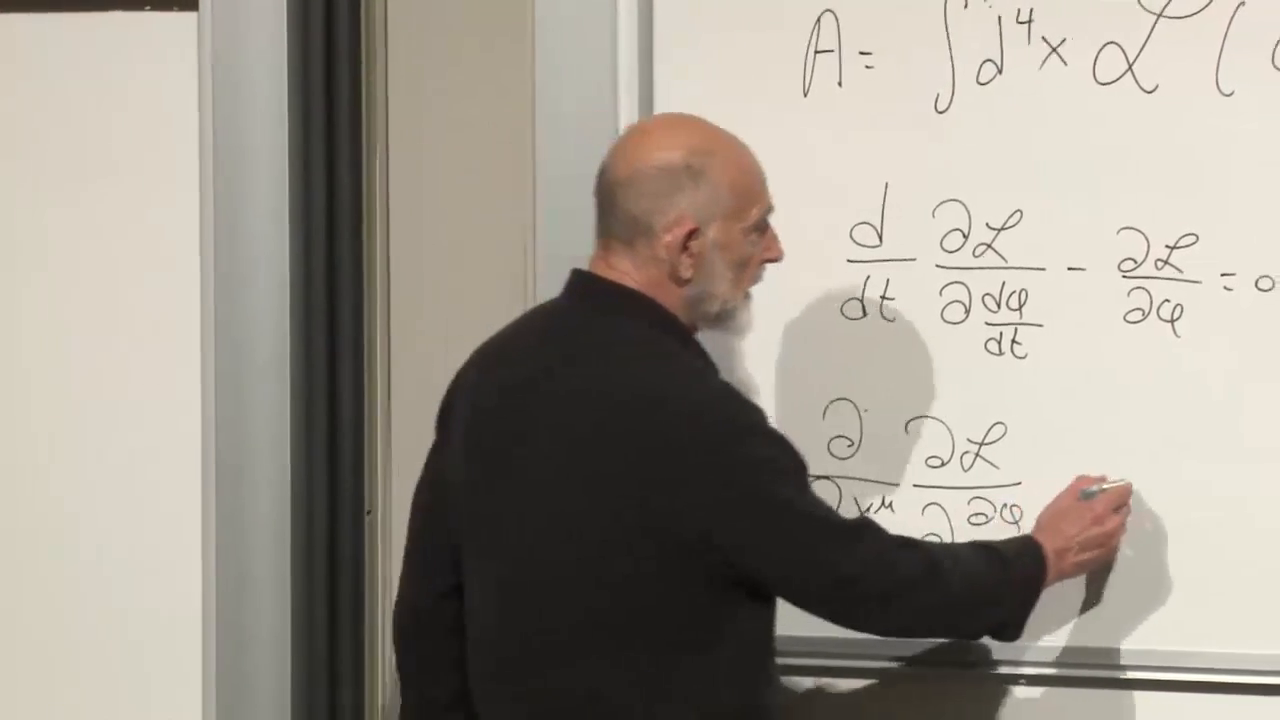
\includegraphics[width=0.90\textwidth]{lecture_04_figure_03.png}
\caption{История скалярного поля, изображенная как поверхность над \(1+1\)-мерной плоскостью пространства-времени.}
\lectureframe{00:20:46}
\end{figure}

Наше физическое пространство-время называют \(3+1\)-мерным: три измерения пространства и одно времени. Настольная модель имеет размерность \(2+1\), а бусины, ограниченные движением по проволоке, наводят на мысль о мире \(1+1\). Дополнительная ось, нужная для изображения \(\phi\), делает невозможным точное изображение даже случая \(3+1\), но определение однозначно: полная история сопоставляет каждому событию пространства-времени одно значение \(\phi\).

\subsection{От фиксированных концов к фиксированным граничным данным}

В вариационной задаче для частицы фиксируют два конца и варьируют кривую между ними. Полевой аналог выбирает область пространства-времени, фиксирует \(\phi\) на ее границе и варьирует \(\phi\) внутри. Эта область может быть прямоугольником на \(1+1\)-мерном рисунке или любой подходящей областью в пространстве-времени большей размерности.

\begin{figure}[htbp]
\centering
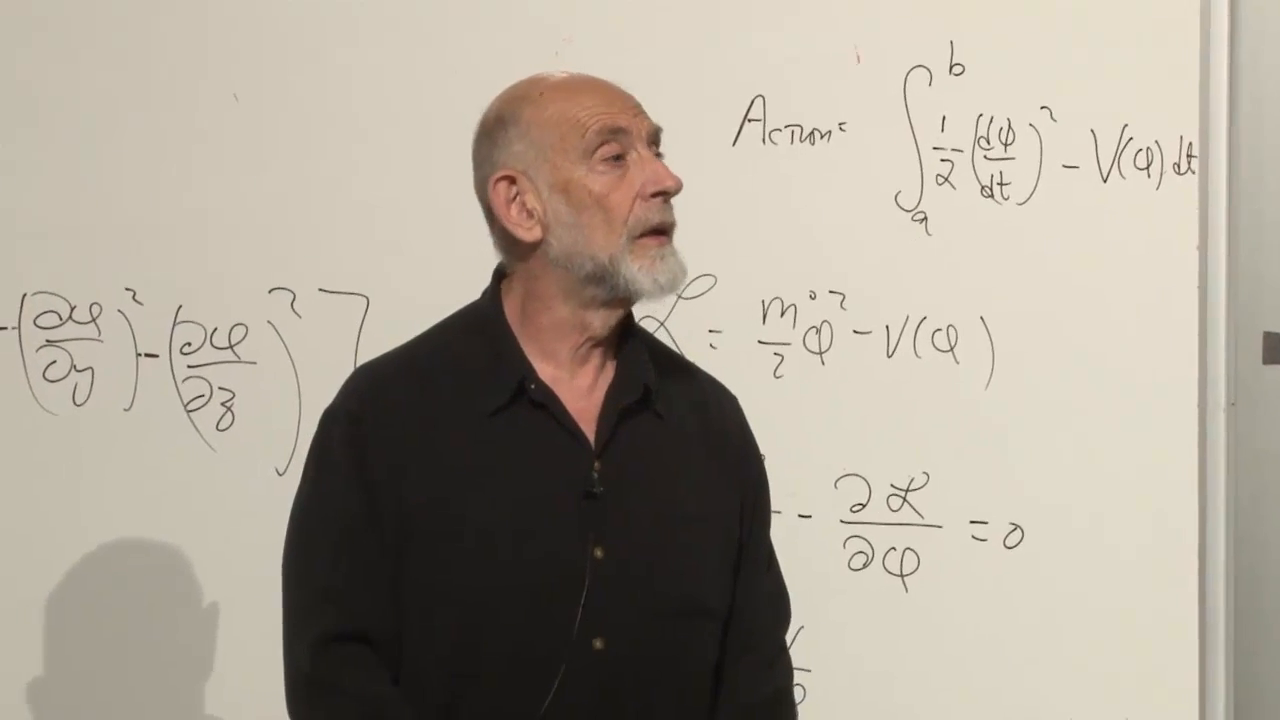
\includegraphics[width=0.90\textwidth]{lecture_04_figure_04.png}
\caption{Область пространства-времени, вся граница которой фиксирована, а поле внутри варьируется.}
\lectureframe{00:24:52}
\end{figure}

\begin{classroomqa}
\audiencequestion{Работает ли лагранжева формулировка, когда потенциал явно зависит от времени?}
\lecturerresponse{Да. Формулировки Эйлера--Лагранжа и Гамильтона по-прежнему работают. Теряется, вообще говоря, сохранение энергии: явная зависимость от времени нарушает симметрию относительно сдвигов по времени. Соответствующее утверждение в теории поля состоит в том, что явная зависимость от пространства-времени допустима, хотя она и влияет на связанные с ней законы сохранения. \lecturetimestamp{00:23:49}}
\end{classroomqa}

\begin{classroomqa}
\audiencequestion{Для прямоугольной области поля фиксируются только верх и низ или вся граница?}
\lecturerresponse{Для этой вариационной конструкции фиксируется вся граница: все четыре стороны в \(1+1\)-мерном прямоугольнике. Полю разрешено колебаться только внутри. Это прямой аналог фиксации обоих концов в механике частицы. \lecturetimestamp{00:24:24}}
\end{classroomqa}

Фиксация всей границы — это утверждение о вариации, используемой для вывода уравнений. Когда полученное гиперболическое уравнение поля рассматривают как задачу физической эволюции, обычно задают подходящие начальные данные и позволяют уравнению распространять их вперед во времени.

\section{Действие и уравнение Эйлера--Лагранжа для поля}

\subsection{Плотность лагранжиана}

Разобьем область пространства-времени на малые ячейки. Предполагается, что действие представляет собой сумму локальных вкладов, по одному от каждой ячейки. В пределе континуума эта сумма превращается в интеграл по пространству-времени:
\begin{equation}
A[\phi]
=
\int_{\Omega} d^4x\,
\mathcal{L}\!\left(
\phi,\partial_\mu\phi;x^\mu
\right),
\qquad
d^4x=dt\,dx\,dy\,dz.
\label{eq:sr4-field-action}
\end{equation}
Величина \(\mathcal{L}\) есть плотность лагранжиана. Точка с запятой в \(\mathcal{L}(\phi,\partial_\mu\phi;x^\mu)\) отделяет динамические аргументы от возможной явной зависимости от координат. В однородной замкнутой системе эта последняя зависимость обычно отсутствует, но вариационный формализм ее не запрещает.

Компактное обозначение
\begin{equation}
\partial_\mu\phi
\equiv
\frac{\partial\phi}{\partial x^\mu}
\end{equation}
объединяет производную по времени и пространственные производные. В используемой на лекции покомпонентной записи вместо этого можно написать
\begin{equation}
\begin{aligned}
\phi_t&=\frac{\partial\phi}{\partial t},\\
\phi_x&=\frac{\partial\phi}{\partial x},\\
\phi_y&=\frac{\partial\phi}{\partial y},\\
\phi_z&=\frac{\partial\phi}{\partial z}.
\end{aligned}
\label{eq:sr4-component-derivatives}
\end{equation}
Полей может быть несколько, так же как у частицы может быть несколько координат. Пока имеется только одно поле \(\phi\).

Обозначение \(d^4x\) — лишь сокращение для меры по четырём координатам. В пространстве-времени другой размерности оно заменялось бы на \(d^Dx\). В прототипе размерности \(0+1\), \(D=1\), и \(d^1x\) — это просто \(dt\).

\begin{figure}[htbp]
\centering
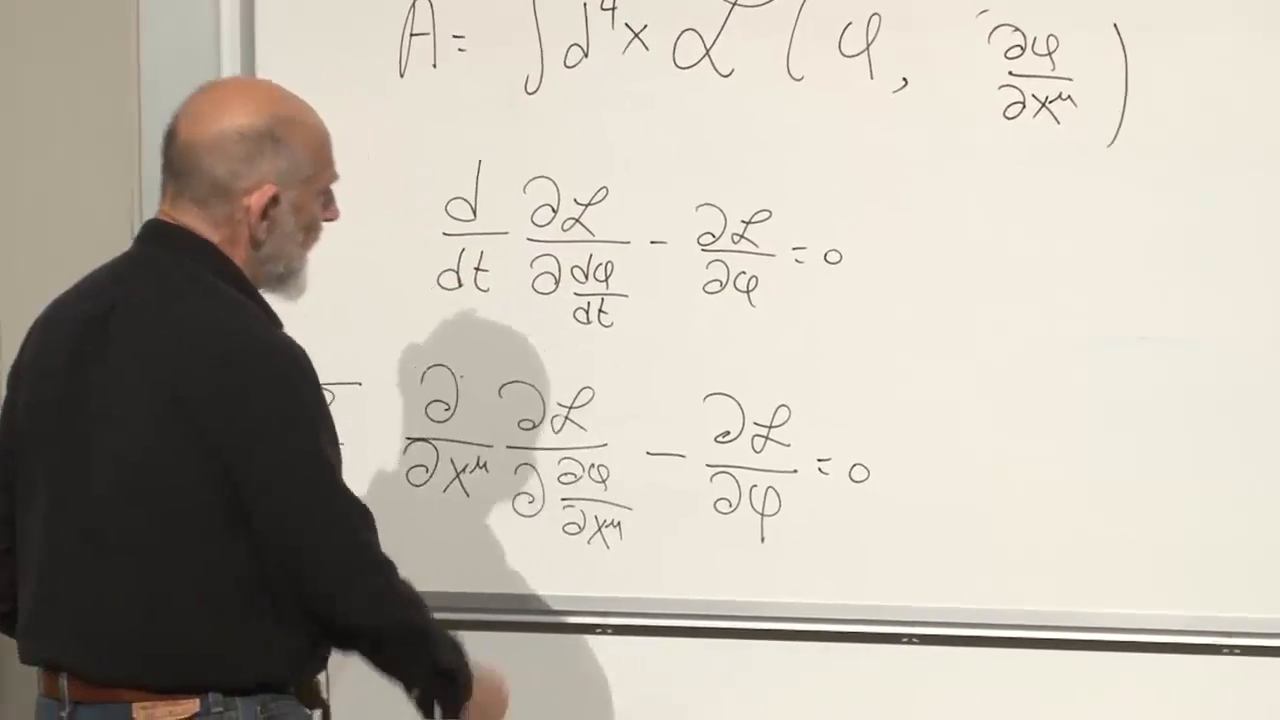
\includegraphics[width=0.90\textwidth]{lecture_04_figure_05.png}
\caption{Плотность действия, записанная как локальная функция поля \(\phi\) и его пространственно-временных производных.}
\lectureframe{00:32:51}
\end{figure}

\begin{classroomqa}
\audiencequestion{Может ли плотность лагранжиана зависеть также и от самих \(x,y,z\)?}
\lecturerresponse{Может, так же как лагранжиан частицы может явно зависеть от \(t\). Для замкнутой системы, инвариантной относительно трансляций, обычно этого нет, но явная зависимость от координат не делает формализм некорректным. \lecturetimestamp{00:30:29}}
\end{classroomqa}

\begin{classroomqa}
\audiencequestion{Относится ли построение до сих пор именно к скалярному полю, или оно является общим?}
\lecturerresponse{Пока вариационная схема является общей. Запись только одной компоненты наводит на мысль о скалярном поле. Векторное поле или набор полей несли бы дополнительные индексы компонентов, и варьировать пришлось бы каждую компоненту. \lecturetimestamp{00:31:00}}
\end{classroomqa}

\subsection{Решёточная картина}

На мелкой пространственно-временной решётке производные превращаются в конечные разности между соседними значениями поля. Тогда действие становится обычной функцией многих переменных. Сетка с 10 точками в одном направлении и 8 в другом уже даёт 80 полевых переменных. При измельчении сетки их число растёт, но правило минимизации остаётся элементарным: продифференцировать действие по значению поля в каждом внутреннем узле и приравнять результат к нулю.

\begin{figure}[htbp]
\centering
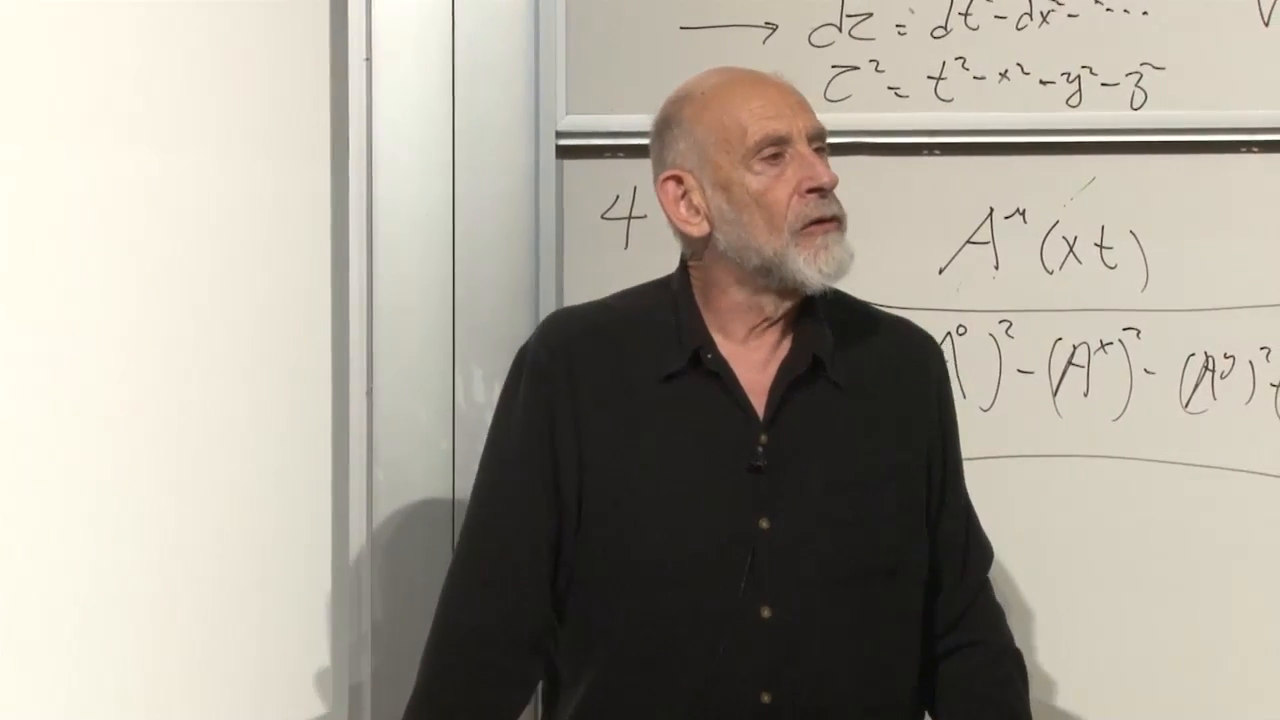
\includegraphics[width=0.90\textwidth]{lecture_04_figure_06.png}
\caption{Область пространства-времени, разбитая на ячейки, так что до перехода к континуальному пределу действие становится обычной функцией многих переменных.}
\lectureframe{00:34:05}
\end{figure}

При переходе к континуальному пределу получается уравнение Эйлера--Лагранжа для поля,
\begin{equation}
\boxed{
\partial_\mu
\left[
\frac{\partial\mathcal{L}}
{\partial(\partial_\mu\phi)}
\right]
-
\frac{\partial\mathcal{L}}{\partial\phi}
=0
}.
\label{eq:sr4-field-el}
\end{equation}
По повторяющемуся индексу \(\mu\) ведётся суммирование по всем направлениям пространства-времени. Если записать то же уравнение без сокращённого обозначения суммирования, получим
\begin{align}
&
\frac{\partial}{\partial t}
\left(\frac{\partial\mathcal{L}}{\partial\phi_t}\right)
+
\frac{\partial}{\partial x}
\left(\frac{\partial\mathcal{L}}{\partial\phi_x}\right)
+
\frac{\partial}{\partial y}
\left(\frac{\partial\mathcal{L}}{\partial\phi_y}\right)
\nonumber\\
&\hspace{3em}
+
\frac{\partial}{\partial z}
\left(\frac{\partial\mathcal{L}}{\partial\phi_z}\right)
-
\frac{\partial\mathcal{L}}{\partial\phi}
=0.
\label{eq:sr4-field-el-expanded}
\end{align}
Первый член — это привычный член для частицы. Теория поля добавляет аналогичный член для каждого пространственного направления. Последний член, \(-\partial\mathcal{L}/\partial\phi\), остаётся без изменений.

\begin{figure}[htbp]
\centering
\includegraphics[width=0.90\textwidth]{lecture_04_figure_07.png}
\caption{Одномерное уравнение Эйлера--Лагранжа и его пространственно-временное обобщение, записанные одно под другим.}
\lectureframe{00:38:44}
\end{figure}

Эту область также называют механикой сплошных сред. В зависимости от степеней свободы одна и та же математика может описывать течение жидкости, упругие смещения или другую сплошную среду.

\begin{classroomqa}
\audiencequestion{Работали бы те же уравнения в мире, где есть пространство, но нет времени?}
\lecturerresponse{Да, как чисто пространственная вариационная задача. Физически именно так ищут статическое решение: предполагают, что поле не зависит от времени, отбрасывают все производные по времени и решают оставшиеся пространственные уравнения. Примером служит не зависящая от времени электрическая или магнитная конфигурация. \lecturetimestamp{00:40:05}}
\end{classroomqa}

\section{Поиск простейшей скалярной динамики}

\subsection{Почему все знаки не могут быть одинаковыми}

Вернёмся к кинетическому члену частицы \(\tfrac12\dot\phi^2\), положим его несущественный общий коэффициент равным единице и попробуем обобщить его. Первой догадкой могло бы быть
\begin{equation}
\mathcal{L}_{+}
=
\frac12
\left[
\phi_t^2+\phi_x^2+\phi_y^2+\phi_z^2
\right].
\label{eq:sr4-all-plus}
\end{equation}
Это полезный ложный ход. Здесь время и пространство входят с одинаковыми знаками. Получающееся уравнение не имело бы гиперболической структуры волнового распространения. В правильной релятивистской комбинации знак при времени один, а при пространстве — противоположный.

\begin{classroomqa}
\audiencequestion{Неверно ли выражение со всеми плюсами потому, что лагранжиан должен быть релятивистски инвариантным?}
\lecturerresponse{Это более глубокий ответ, и он верен. На лекции до нужного знака сначала доходят более примитивным способом: волны различают эволюцию во времени и изменение в пространстве, поэтому время не может входить точно так же, как ещё одна пространственная координата. Инвариантность Лоренца вскоре превратит эту интуицию в точное правило. \lecturetimestamp{00:43:19}}
\end{classroomqa}

Восстановив характерную скорость \(c\), получаем простую скалярную плотность лагранжиана:
\begin{equation}
\boxed{
\mathcal{L}
=
\frac12
\left[
\frac{1}{c^2}\phi_t^2
-\phi_x^2-\phi_y^2-\phi_z^2
\right]
-V(\phi)
}.
\label{eq:sr4-scalar-lagrangian}
\end{equation}
Для релятивистского поля \(c\) — это скорость света. В модели сплошной среды это могла бы быть скорость звука, скорость упругой волны или другая характерная скорость распространения.

Общий множитель \(1/2\) является условным, как и в \(\tfrac12m\dot\phi^2\). Умножение всего действия на ненулевую константу не меняет его экстремали; этот выбор фиксирует названия и нормировку параметров в уравнениях. После выбора этой нормировки её нужно использовать последовательно.

\begin{classroomqa}
\audiencequestion{Можно ли считать члены с пространственным градиентом частью потенциальной энергии?}
\lecturerresponse{Да. В записи вида «кинетическая минус потенциальная» кинетическая часть содержит производные по времени. Члены без производных по времени, включая пространственные градиенты и \(V(\phi)\), относятся к потенциальной части. Окончательная причина их относительного знака в релятивистской теории — лоренцева метрика. \lecturetimestamp{00:45:37}}
\end{classroomqa}

\subsection{Волновое уравнение}

Применим \eqref{eq:sr4-field-el}. Члены с производными имеют вид
\begin{equation}
\frac{\partial\mathcal{L}}{\partial\phi_t}
=\frac{1}{c^2}\phi_t,
\qquad
\frac{\partial\mathcal{L}}{\partial\phi_i}
=-\phi_i,
\end{equation}
тогда как
\begin{equation}
\frac{\partial\mathcal{L}}{\partial\phi}
=-\frac{dV}{d\phi}.
\end{equation}
Следовательно,
\begin{equation}
\begin{aligned}
&\boxed{
\frac{1}{c^2}\frac{\partial^2\phi}{\partial t^2}
-\nabla^2\phi
+\frac{dV}{d\phi}
=0
},\\[0.5em]
\nabla^2
&=
\frac{\partial^2}{\partial x^2}
+\frac{\partial^2}{\partial y^2}\\
&\quad
+\frac{\partial^2}{\partial z^2}.
\end{aligned}
\label{eq:sr4-general-scalar-eom}
\end{equation}

Если \(V=0\), это сводится к
\begin{equation}
\boxed{
\frac{1}{c^2}\phi_{tt}-\nabla^2\phi=0
},
\label{eq:sr4-wave-equation}
\end{equation}
то есть к волновому уравнению. На лекции это уравнение узнают, но откладывают его решение. Его решения распространяют возмущения со скоростью \(c\).

\begin{figure}[htbp]
\centering
\includegraphics[width=0.90\textwidth]{lecture_04_figure_08.png}
\caption{Одномерная форма \(c^{-2}\phi_{tt}-\phi_{xx}=0\), распознаваемая как волновое уравнение.}
\lectureframe{00:50:30}
\end{figure}

\subsection{Поле связанных гармонических осцилляторов}

Теперь выберем квадратичный потенциал,
\begin{equation}
V(\phi)=\frac12\mu^2\phi^2,
\qquad
\frac{dV}{d\phi}=\mu^2\phi.
\label{eq:sr4-quadratic-potential}
\end{equation}
Если бы \(\phi\) было координатой частицы, это был бы потенциал гармонического осциллятора с коэффициентом жёсткости \(\mu^2\). Для поля
\begin{equation}
\boxed{
\frac{1}{c^2}\phi_{tt}-\nabla^2\phi+\mu^2\phi=0
}.
\label{eq:sr4-klein-gordon}
\end{equation}
Если отбросить пространственную производную, это просто уравнение: ускорение плюс константа, умноженная на смещение, равно нулю. Градиент связывает соседние точки, превращая осциллятор в континуум, в котором могут распространяться волны. В релятивистской теории поля \eqref{eq:sr4-klein-gordon} называется массивным уравнением Клейна--Гордона; классически \(\mu\) — это обратный масштаб длины, который модифицирует распространение волн.

\begin{figure}[htbp]
\centering
\includegraphics[width=0.90\textwidth]{lecture_04_figure_09.png}
\caption{Квадратичный потенциал и возникающее волновое уравнение с восстанавливающим членом \(\mu^2\phi\).}
\lectureframe{00:52:38}
\end{figure}

\begin{classroomqa}
\audiencequestion{Почему множитель \(1/2\) в \(V=\tfrac12\mu^2\phi^2\) исчезает из уравнения движения?}
\lecturerresponse{Дифференцирование \(\phi^2\) даёт множитель 2. Обычный \(1/2\) вводится именно для того, чтобы \(dV/d\phi=\mu^2\phi\), точно так же как \(V(x)=\tfrac12kx^2\) даёт восстанавливающую силу \(-kx\). \lecturetimestamp{00:53:17}}
\end{classroomqa}

Уравнение линейно: \(\phi\) и каждая из его производных входят только в первой степени. Члены вроде \(\phi^2\) или \(\phi\,\partial_\mu\phi\) в уравнении движения сделали бы динамику нелинейной.

\section{Скаляры Лоренца и четырёхвекторы}

\subsection{Действие должно быть независимо от системы отсчёта}

Один лишь вариационный аппарат задаёт много возможных теорий поля. Теория относительности накладывает дополнительное требование: действие должно иметь одно и то же значение и один и тот же вид во всякой инерциальной системе отсчёта. Для свободной частицы этого достигали, интегрируя инвариантное собственное время \(d\tau\) вдоль мировой линии. Для поля действие интегрируется по пространству-времени, поэтому его локальные составляющие должны преобразовываться соответствующим образом.

При собственном преобразовании Лоренца мера пространства-времени инвариантна, \(d^4x'=d^4x\). Поэтому достаточно потребовать, чтобы плотность лагранжиана была скаляром Лоренца:
\begin{equation}
\mathcal{L}'(x')=\mathcal{L}(x).
\label{eq:sr4-lagrangian-scalar}
\end{equation}

\subsection{Скалярные поля}

Для скалярного поля выполняется
\begin{equation}
\boxed{\phi'(x')=\phi(x)}.
\label{eq:sr4-scalar-transform}
\end{equation}
Координаты \(x\) и \(x'\) обозначают одно и то же событие в двух системах отсчёта. Функциональные выражения, которыми пользуются наблюдатели, могут выглядеть по-разному, но число, приписываемое этому физическому событию, одно и то же.

\begin{figure}[htbp]
\centering
\includegraphics[width=0.90\textwidth]{lecture_04_figure_10.png}
\caption{Определяющий закон преобразования скалярного поля: \(\phi(x)=\phi'(x')\).}
\lectureframe{00:59:33}
\end{figure}

Первоначальную интуицию давала температура, хотя движущийся термометр в материальной среде не является идеальным релятивистским примером. Существенно именно определение \eqref{eq:sr4-scalar-transform}, а не аналогия с термометром.

\subsection{Четырехвекторы}

В единицах \(c=1\) буст со скоростью \(v\) вдоль оси \(x\) имеет вид
\begin{equation}
\begin{aligned}
t'&=\gamma(t-vx),\\
x'&=\gamma(x-vt),\\
y'&=y,\\
z'&=z,\\
\gamma&=\frac{1}{\sqrt{1-v^2}}.
\end{aligned}
\label{eq:sr4-x-boost}
\end{equation}

\begin{figure}[htbp]
\centering
\includegraphics[width=0.90\textwidth]{lecture_04_figure_11.png}
\caption{Преобразование Лоренца для буста вдоль оси \(x\) в единицах \(c=1\).}
\lectureframe{01:02:26}
\end{figure}

Любые четыре величины, которые при бустах смешиваются одинаковым образом, образуют четырехвектор.
Уже встречавшиеся примеры — это \(x^\mu\), \(dx^\mu\) и четырехскорость
\(u^\mu=dx^\mu/d\tau\). Умножение четырехвектора на скаляр дает другой
четырехвектор. Движущаяся релятивистская жидкость дает пример поля:
ее четырехскорость \(u^\mu(x)\) может различаться от события к событию.

Для того же буста, что и в \eqref{eq:sr4-x-boost}, произвольный четырехвектор преобразуется по закону
\begin{equation}
\begin{aligned}
A'^0&=\gamma(A^0-vA^x),\\
A'^x&=\gamma(A^x-vA^0),\\
A'^y&=A^y,\\
A'^z&=A^z.
\end{aligned}
\label{eq:sr4-vector-boost}
\end{equation}

Для произвольного четырехвектора \(A^\mu=(A^0,A^x,A^y,A^z)\) лоренцева норма
\begin{equation}
\boxed{
A_\mu A^\mu
=(A^0)^2-(A^x)^2-(A^y)^2-(A^z)^2
}
\label{eq:sr4-vector-norm}
\end{equation}
является скаляром. Она инвариантна по той же алгебраической причине, по которой инвариантно
\begin{equation}
d\tau^2=dt^2-dx^2-dy^2-dz^2
\end{equation}
На лекции ненадолго заканчиваются неиспользованные буквы для обозначения произвольного
вектора, прежде чем в итоге выбирается \(A\); помогает ассоциация \(A\) с английским словом arrow.

\begin{figure}[htbp]
\centering
\includegraphics[width=0.90\textwidth]{lecture_04_figure_12.png}
\caption{Общее четырехвекторное поле и лоренцева разность квадратов, из которой строится его инвариантная норма.}
\lectureframe{01:09:06}
\end{figure}

\subsection{Производная скаляра}

Дифференцирование скаляра по четырем координатам пространства-времени
дает четыре компонента
\begin{equation}
\partial_\mu\phi
=
\left(
\frac{\partial\phi}{\partial t},
\frac{\partial\phi}{\partial x},
\frac{\partial\phi}{\partial y},
\frac{\partial\phi}{\partial z}
\right)
\qquad(c=1).
\end{equation}
Строго говоря, \(\partial_\mu\phi\) — это ковектор; метрика Минковского поднимает его
индекс, превращая его в \(\partial^\mu\phi\). Здесь в рассуждении по компонентам это различие безвредно, но оно однозначно фиксирует свертку:
\begin{equation}
\boxed{
\partial_\mu\phi\,\partial^\mu\phi
=
\frac{1}{c^2}\phi_t^2
-\phi_x^2-\phi_y^2-\phi_z^2
}.
\label{eq:sr4-derivative-scalar}
\end{equation}

\begin{figure}[htbp]
\centering
\includegraphics[width=0.90\textwidth]{lecture_04_figure_13.png}
\caption{Инвариантная разность квадратов, построенная из первых производных скалярного поля.}
\lectureframe{01:13:55}
\end{figure}

\begin{classroomqa}
\audiencequestion{Является ли эта комбинация производных лапласианом?}
\lecturerresponse{Нет. Показанный инвариант квадратичен по первым производным. Лапласиан содержит вторые пространственные производные. Вторые производные появляются только после варьирования действия, в волновом уравнении. \lecturetimestamp{01:13:22}}
\end{classroomqa}

Теперь знаковая структура в \eqref{eq:sr4-scalar-lagrangian} не угадывается, а объясняется. Комбинация кинетического и градиентного членов является лоренцевым скаляром
\(\partial_\mu\phi\,\partial^\mu\phi\). Поэтому простейшая квадратичная теория имеет вид
\begin{equation}
\mathcal{L}
=
\frac12\partial_\mu\phi\,\partial^\mu\phi
-\frac12\mu^2\phi^2.
\label{eq:sr4-covariant-lagrangian}
\end{equation}

\begin{figure}[htbp]
\centering
\includegraphics[width=0.90\textwidth]{lecture_04_figure_14.png}
\caption{Полный квадратичный лагранжиан скалярного поля и его линейное полевое уравнение, выписанные на доске.}
\lectureframe{01:19:12}
\end{figure}

\section{Насколько велика свобода?}

Когда известно правило построения скаляров, возможными становятся многие лагранжианы.
Поле \(\phi\) является скаляром, поэтому любая обычная функция \(F(\phi)\) тоже
является скаляром: \(\phi^2\), \(\phi^3\), \(\cosh\phi\) и так далее. Допустимы
и численные параметры. Символ вроде \(\mu\) можно ввести как
постоянный коэффициент; остаются только вопросы о его размерности и его
физической интерпретации.

\begin{classroomqa}
\audiencequestion{Можно ли ввести массу в лагранжиан?}
\lecturerresponse{Постоянный параметр, конечно, можно. На этом этапе следует спросить, массой какого объекта он является, потому что \(\mu\) в классической теории поля — просто число, пока не выяснен его физический смысл. В квадратичной релятивистской скалярной теории оно задает масштаб массы или обратной длины. \lecturetimestamp{01:14:16}}
\end{classroomqa}

Скаляры можно перемножать:
\begin{equation}
F(\phi)\,\partial_\mu\phi\,\partial^\mu\phi
\end{equation}
лоренц-инвариантен. Сам производный скаляр тоже можно возвести в квадрат, получая
более высокие степени первых производных. Можно рассматривать и высшие
производные, хотя в лекции внимание ограничивается полями и их первыми
производными — стандартной схемой, приводящей к уравнениям движения второго
порядка. Теории с высшими производными требуют дополнительной осторожности, потому что
они, как правило, вводят дополнительные динамические данные и возможные неустойчивости.

\begin{classroomqa}
\audiencequestion{Является ли конструкция в виде разности квадратов действительно метрикой пространства-времени?}
\lecturerresponse{Да. Метрика при выбранной сигнатуре имеет вид \(dt^2-dx^2-dy^2-dz^2\). В лекции слово метрика пока еще не подчеркивалось, но это в точности та геометрия пространства-времени, которая станет центральной в общей теории относительности. \lecturetimestamp{01:19:39}}
\end{classroomqa}

\begin{classroomqa}
\audiencequestion{Существуют ли объекты более общие, чем четырехвекторы, с компонентами, такими как \(xy\) или \(tx\)?}
\lecturerresponse{Да. Это тензоры. У скаляра нет пространственно-временного индекса, у вектора один, а у тензора ранга два имеются компоненты, например \(T^{xx}\), \(T^{xy}\) и \(T^{tx}\). В большей части нынешнего обсуждения скалярного поля они не нужны; в общей теории относительности без них не обойтись. \lecturetimestamp{01:20:49}}
\end{classroomqa}

\begin{classroomqa}
\audiencequestion{Почему обсуждаются только бусты, смешивающие \(t\) с \(x\)? Может ли буст быть направлен в другую сторону и иначе смешивать пространственные оси?}
\lecturerresponse{Конечно. Буст вдоль \(y\) смешивает \(t\) с \(y\) и оставляет \(x,z\) неизменными. Общее преобразование Лоренца можно составить из пространственных вращений и буста вдоль выбранной оси. Следовательно, достаточно установить инвариантность относительно вращений и относительно буста вдоль одной стандартной оси. \lecturetimestamp{01:22:06}}
\end{classroomqa}

\begin{classroomqa}
\audiencequestion{При таком большом числе возможных скалярных комбинаций описывают ли все получающиеся лагранжианы осмысленную физику?}
\lecturerresponse{На классическом уровне свобода огромна, хотя и ограничена дополнительными требованиями, такими как разумные знаки, локальность и корректно поставленная задача эволюции. Гораздо меньшее число произвольных выборов задает корректные фундаментальные квантовые теории. Современная эффективная теория поля допускает много дополнительных взаимодействий ниже масштаба отсечки, но тогда необходимо указать область их применимости. \lecturetimestamp{01:27:57}}
\end{classroomqa}

\begin{classroomqa}
\audiencequestion{Должно ли поле быть непрерывным?}
\lecturerresponse{Для гладких теорий, которые здесь обсуждаются, да. Разрыв порождает сингулярные производные и при квадратичном градиентном члене обычно бесконечные действие и энергию. Более сингулярные конфигурации можно рассматривать только при наличии дополнительной математической структуры; это не те обычные поля конечной энергии, которые здесь строятся. \lecturetimestamp{01:29:29}}
\end{classroomqa}

\section{Частица, связанная со скалярным полем}

\subsection{Снова о свободной частице}

В заключительной части лекции частицы и поля объединяются на классическом
уровне. Это еще не квантовое утверждение о том, что частицы являются возбуждениями
полей. Вместо этого предположим, что кто-то уже нашел фоновое
скалярное поле \(\phi(x,t)\), и спросим, как частица движется в нем.

Для свободной релятивистской частицы
\begin{equation}
A_{\rm free}=-m\int d\tau.
\label{eq:sr4-free-particle-action}
\end{equation}
В одном пространственном измерении и при \(c=1\)
\begin{equation}
d\tau=dt\sqrt{1-\dot x^2},
\qquad
L_{\rm free}=-m\sqrt{1-\dot x^2}.
\label{eq:sr4-free-particle-l}
\end{equation}
Знак минус выбран так, чтобы разложение при малых скоростях давало обычный
положительный ньютоновский кинетический член:
\begin{equation}
L_{\rm free}
\approx -m+\frac12m\dot x^2+\cdots.
\end{equation}

\begin{figure}[htbp]
\centering
\includegraphics[width=0.90\textwidth]{lecture_04_figure_15.png}
\caption{Инвариантное действие свободной частицы, переписанное как лагранжиан в координатном времени.}
\lectureframe{01:34:31}
\end{figure}

\subsection{Простейшая скалярная связь}

И \(d\tau\), и \(\phi\) являются скалярами. Поэтому простейшая линейная связь
имеет вид
\begin{equation}
\boxed{
A
=
\int d\tau\,[-m+\phi(x,t)]
}.
\label{eq:sr4-coupled-action}
\end{equation}
Этот выбор не единственный. \(\phi\) можно заменить любой функцией
\(F(\phi)\). Линейного члена достаточно, чтобы показать физическую идею.

\begin{figure}[htbp]
\centering
\includegraphics[width=0.90\textwidth]{lecture_04_figure_16.png}
\caption{Свободное действие, дополненное простейшей лоренц-инвариантной скалярной связью.}
\lectureframe{01:37:21}
\end{figure}

\begin{classroomqa}
\audiencequestion{Должно ли \(\phi\) оставаться под знаком интеграла?}
\lecturerresponse{Да. Поле вычисляется на мировой линии частицы, \(\phi(x(t),t)\), и вообще говоря меняется от одной точки траектории к другой. Даже если фон не зависит явно от времени, \(\phi=\phi(x)\), оно все равно меняется со временем, когда частица движется в пространстве. Вынести его наружу можно было бы только в том случае, если вдоль пути поле постоянно. \lecturetimestamp{01:37:47}}
\end{classroomqa}

\begin{classroomqa}
\audiencequestion{Означает ли \(x\) в \(\phi(x,t)\) положение частицы?}
\lecturerresponse{Да. Это \(x=x(t)\), положение частицы в момент \(t\). Действие берет значения заданного пространственно-временного поля вдоль этой траектории. \lecturetimestamp{01:38:08}}
\end{classroomqa}

Для одномерного движения \eqref{eq:sr4-coupled-action} дает
\begin{equation}
L
=
-(m-\phi(x,t))\sqrt{1-\dot x^2}.
\label{eq:sr4-coupled-lagrangian}
\end{equation}
Скалярный фон появляется в точности на том месте, которое занимает масса покоя:
\begin{equation}
m_{\rm eff}(x,t)=m-\phi(x,t).
\label{eq:sr4-effective-mass}
\end{equation}
Если \(\phi\) становится почти постоянным ненулевым значением, частица ведет себя
так, как если бы ее масса изменилась. Это лишь классическая игрушечная модель, а не полный
механизм Хиггса, но она передает тот самый вкус идеи Хиггса: скалярный фон может входить в динамику частицы как массовый член.

\subsection{Уравнение для частицы}

Канонический импульс равен
\begin{equation}
p
=
\frac{\partial L}{\partial\dot x}
=
(m-\phi)
\frac{\dot x}{\sqrt{1-\dot x^2}}.
\label{eq:sr4-coupled-momentum}
\end{equation}

\begin{figure}[htbp]
\centering
\includegraphics[width=0.90\textwidth]{lecture_04_figure_17.png}
\caption{Скалярный фон заменяет \(m\) на \(m-\phi(x,t)\) в релятивистском каноническом импульсе.}
\lectureframe{01:43:38}
\end{figure}

Производная лагранжиана по координате равна
\begin{equation}
\frac{\partial L}{\partial x}
=
\frac{\partial\phi}{\partial x}
\sqrt{1-\dot x^2}.
\end{equation}
Поскольку знак фиксируется действием
\eqref{eq:sr4-coupled-action}, уравнение Эйлера--Лагранжа поэтому имеет вид
\begin{equation}
\boxed{
\frac{d}{dt}
\left[
(m-\phi)
\frac{\dot x}{\sqrt{1-\dot x^2}}
\right]
=
\frac{\partial\phi}{\partial x}
\sqrt{1-\dot x^2}
}.
\label{eq:sr4-coupled-eom}
\end{equation}

\begin{figure}[htbp]
\centering
\includegraphics[width=0.90\textwidth]{lecture_04_figure_18.png}
\caption{Связанное уравнение, собранное из импульса и пространственной производной фонового поля; действие фиксирует окончательный знак в \eqref{eq:sr4-coupled-eom}.}
\lectureframe{01:45:24}
\end{figure}

\begin{classroomqa}
\audiencequestion{Почему в \(\partial\phi/\partial x\) сохраняется множитель \(\sqrt{1-\dot x^2}\)?}
\lecturerresponse{Потому что по \(x\) дифференцируется только множитель \(\phi(x,t)\). В лагранжиане корень его умножает и не зависит от координаты, если при взятии частной производной \(\dot x\) удерживается фиксированным, поэтому корень остается. \lecturetimestamp{01:45:50}}
\end{classroomqa}

Раскрывая полную производную по времени, получаем
\begin{align}
&(m-\phi)
\frac{d}{dt}
\left(
\frac{\dot x}{\sqrt{1-\dot x^2}}
\right)
-
\dot\phi\,
\frac{\dot x}{\sqrt{1-\dot x^2}}
\nonumber\\
&\hspace{10em}
=
\frac{\partial\phi}{\partial x}
\sqrt{1-\dot x^2}.
\label{eq:sr4-coupled-expanded}
\end{align}
Если фон статичен, \(\phi=\phi(x)\), его производная вдоль движущейся мировой линии не равна нулю. Правило цепочки дает
\begin{equation}
\boxed{
\dot\phi
=
\frac{d}{dt}\phi(x(t))
=
\frac{\partial\phi}{\partial x}\dot x
}.
\label{eq:sr4-chain-rule}
\end{equation}

\begin{classroomqa}
\audiencequestion{Если у \(\phi\) нет явной зависимости от времени, почему \(\dot\phi\) не равно нулю?}
\lecturerresponse{Потому что частица меняет положение. Поле берется в точке \(x(t)\), поэтому его полная производная равна \(\dot\phi=\phi_x\dot x\). Статическое поле означает \(\partial\phi/\partial t=0\), а не то, что всякая движущаяся частица видит постоянное значение поля. \lecturetimestamp{01:48:10}}
\end{classroomqa}

\begin{figure}[htbp]
\centering
\includegraphics[width=0.90\textwidth]{lecture_04_figure_19.png}
\caption{Позднее разложение связанного уравнения после применения правила цепочки вдоль мировой линии.}
\lectureframe{01:49:11}
\end{figure}

Точное выражение не особенно красиво, и лекция не делает вид, будто это не так. Тем не менее его предел при малых скоростях хорошо знаком. Поскольку
\(\sqrt{1-\dot x^2}\approx1\), уравнение в ведущем порядке имеет вид
\begin{equation}
\frac{d}{dt}\bigl[(m-\phi)\dot x\bigr]
\approx
\frac{\partial\phi}{\partial x}.
\end{equation}
Если изменение эффективной массы тоже рассматривать как возмущение, это переходит в
\begin{equation}
(m-\phi)\ddot x
\approx
\frac{\partial\phi}{\partial x}.
\label{eq:sr4-nonrel-force}
\end{equation}
В самом деле, лагранжиан при малых скоростях равен
\begin{equation}
L
\approx
-m+\phi+\frac12(m-\phi)\dot x^2,
\end{equation}
так что в ведущем порядке потенциальная энергия есть \(U=-\phi\), а сила равна
\(-dU/dx=\partial_x\phi\). Восстановить множители \(c\) и вновь получить эту ньютоновскую картину — упражнение, которым завершается лекция.

Путь от частиц к полям теперь завершен. История частицы
\(\phi(t)\) дала \(0+1\)-мерный прототип; история поля
\(\phi(x)\) превратила действие в пространственно-временной интеграл; полевое
уравнение Эйлера--Лагранжа породило волновую динамику; скаляры Лоренца задали релятивистскую структуру знаков; и тот же инвариантный язык позволил скалярному фону обратно воздействовать на частицу.
